% ridge_trench_overview_v2.tex — SIMPLIFIED v2 (2026-07-09, user-directed): decomposition
% legend removed; bare z0/zc (equipotential note -> caption); 3-line box stacks (the
% F_B~0 and N_D(x_R)~0 assumptions carried by the F_B row and sidewall labels); bare
% sigma_xx on outer walls, x_I arrow pair unlabeled; axes pulled in close.
% Vertically exaggerated; ridge horizontally compressed (axis break). Plate = cooling
% isotherm, thickening from the ridge, asymptoting to constant thickness at the trench.
% Dashed boxes = integration domains of the vertically-integrated stress equilibrium.
% Compile: tectonic ridge_trench_overview.tex
\documentclass[border=8pt]{standalone}
\usepackage{amsmath}
\usepackage{cancel}
\usepackage{tikz}
\usetikzlibrary{decorations.pathmorphing,arrows.meta}
\definecolor{cwater}{HTML}{FFFFFF}
\definecolor{cplate}{HTML}{B7BEC9}
\definecolor{casth}{HTML}{F7E7CE}
\definecolor{cboxA}{HTML}{0072B2}
\definecolor{cboxB}{HTML}{D55E00}
\definecolor{cpush}{HTML}{009E73}
\begin{document}
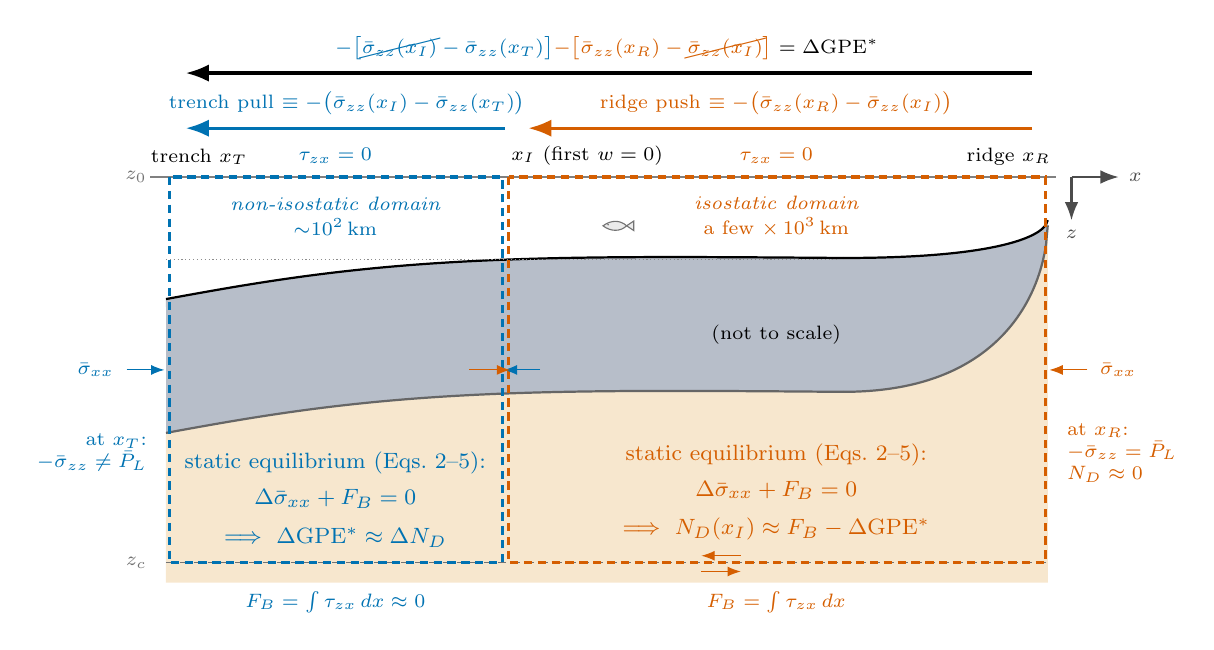
\begin{tikzpicture}[>=Latex,scale=1.0,font=\small]

  % ---- geometry ----
  \def\XI{4.3}        % first isostatic column: b x = pi/2, b = 0.3653
  \def\XJ{8.6}        % junction = forebulge crest (b x = pi): both profiles have zero slope here
  \def\XR{11.2}       % ridge axis
  \def\ZC{-4.9}       % compensation level
  % trench deflection amplitude = ridge subsidence = 0.5 (old-lithosphere equality)
  % plate thickness 1.7
  \def\topoA{-1.05-0.5*exp(-0.3653*\x)*cos(20.93*\x)}
  \def\baseA{-1.05-0.5*exp(-0.3653*\x)*cos(20.93*\x)-1.7}
  % ridge profiles sin(90 sqrt(u)): crest -0.5284 = forebulge height + 0.5; zero slope at XJ
  \def\topoB{-0.5284-0.5*sin(90*sqrt((11.2-\x)/2.6))}
  \def\baseB{-0.5284-2.2*sin(90*sqrt((11.2-\x)/2.6))}

  % ---- fills (continuous domain, no axis break) ----
  \fill[cwater] (0,0) -- plot[domain=0:\XJ,samples=160] (\x,{\topoA})
        -- plot[domain=\XJ:\XR,samples=120] (\x,{\topoB}) -- (\XR,0) -- cycle;
  \fill[cplate] plot[domain=0:\XJ,samples=160] (\x,{\topoA})
        -- plot[domain=\XJ:\XR,samples=120] (\x,{\topoB})
        -- plot[domain=\XR:\XJ,samples=120] (\x,{\baseB})
        -- plot[domain=\XJ:0,samples=160] (\x,{\baseA}) -- cycle;
  \fill[casth] plot[domain=0:\XJ,samples=160] (\x,{\baseA})
        -- plot[domain=\XJ:\XR,samples=120] (\x,{\baseB}) -- (\XR,-5.15) -- (0,-5.15) -- cycle;

  % ---- outlines + reference levels ----
  \draw[thick] plot[domain=0:\XJ,samples=160] (\x,{\topoA});
  \draw[thick] plot[domain=\XJ:\XR,samples=120] (\x,{\topoB});
  \draw[thick,black!60] plot[domain=0:\XJ,samples=160] (\x,{\baseA});
  \draw[thick,black!60] plot[domain=\XJ:\XR,samples=120] (\x,{\baseB});
  \draw[thin,black!50] (-0.2,0) -- (\XR+0.1,0);
  \node[left,black!55] at (-0.12,0) {\scriptsize $z_{0}$};
  \node[black] at (7.75,-2.0) {\scriptsize (not to scale)};
  % top-boundary assumption, one per box, outside the box (symmetric with the F_B row below)
  \node[cboxA,above] at (2.15,0.05) {\scriptsize $\tau_{zx}=0$};
  \node[cboxB,above] at (7.75,0.05) {\scriptsize $\tau_{zx}=0$};
  \draw[densely dotted,black!45] (0,-1.05) -- (8.55,-1.05);   % undeflected seafloor (w=0 reference)
  % a little fish marks the water (sea fill now white)
  \begin{scope}[shift={(5.55,-0.62)},scale=0.2]
    \draw[black!55,fill=black!8]
      (0,0) .. controls (0.5,0.38) and (1.1,0.38) .. (1.5,0)
            .. controls (1.1,-0.38) and (0.5,-0.38) .. (0,0) -- cycle;
    \draw[black!55,fill=black!8] (1.5,0) -- (1.95,0.3) -- (1.95,-0.3) -- cycle;
    \fill[black!65] (0.32,0.07) circle (0.05);
  \end{scope}

  % ---- compensation level ----
  \draw[densely dashed,black!55] (0,\ZC) -- (\XR,\ZC);
  \node[left,black!55] at (-0.12,\ZC) {\scriptsize $z_c$};

  % ---- integration boxes ----
  \draw[cboxA,densely dashed,line width=1.1pt] (0.04,0) rectangle ({\XI-0.03},\ZC);
  \draw[cboxB,densely dashed,line width=1.1pt] ({\XI+0.05},0) rectangle (\XR-0.03,\ZC);
  % box-1: header / balance / approximation / big arrow / final form
  \node[cboxA,align=center] at (2.15,-4.1)
       {\footnotesize static equilibrium (Eqs.~2--5):\\[2pt]
        \footnotesize $\Delta\bar\sigma_{xx}+F_{B}=0$\\[3pt]
        \footnotesize $\Longrightarrow\ \Delta\mathrm{GPE}^{*}\approx\Delta N_{D}$};
  % basal shear traction pair on the orange box (sense per the traction on the domain)
  \draw[->,cboxB,thin] (7.3,{\ZC+0.09}) -- (6.8,{\ZC+0.09});
  \draw[->,cboxB,thin] (6.8,{\ZC-0.11}) -- (7.3,{\ZC-0.11});
  % box-2: header / balance / approximation / big arrow / final form
  \node[cboxB,align=center] at (7.75,-4.0)
       {\footnotesize static equilibrium (Eqs.~2--5):\\[2pt]
        \footnotesize $\Delta\bar\sigma_{xx}+F_{B}=0$\\[3pt]
        \footnotesize $\Longrightarrow\ N_{D}(x_I)\approx F_{B}-\Delta\mathrm{GPE}^{*}$};
  % F_B definitions under the basal boundaries
  \node[cboxA] at (2.15,{\ZC-0.5}) {\scriptsize $F_{B}=\int\tau_{zx}\,dx\approx0$};
  \node[cboxB] at (7.75,{\ZC-0.5}) {\scriptsize $F_{B}=\int\tau_{zx}\,dx$};
  % axis orientation: positive x rightward, positive z down
  \draw[->,thick,black!70] ({\XR+0.3},0) -- ({\XR+0.9},0) node[right]{\scriptsize $x$};
  \draw[->,thick,black!70] ({\XR+0.3},0) -- ({\XR+0.3},-0.55) node[below]{\scriptsize $z$};
  % wall resultants, signed by the outward normal (n_x = -1 left walls, +1 right walls);
  % each box's balance line = sum of its boundary annotations. All arrows at z_c/2.
  \draw[->,cboxA] (-0.5,-2.45) -- (-0.02,-2.45);
  \node[cboxA,left] at (-0.54,-2.45) {\scriptsize $\bar\sigma_{xx}$};
  \draw[->,cboxB] ({\XR+0.5},-2.45) -- ({\XR+0.02},-2.45);
  \node[cboxB,right] at ({\XR+0.54},-2.45) {\scriptsize $\bar\sigma_{xx}$};
  \draw[->,cboxA] ({\XI+0.45},-2.45) -- ({\XI-0.01},-2.45);
  \draw[->,cboxB] ({\XI-0.45},-2.45) -- ({\XI+0.07},-2.45);

  % ---- column labels ----
  \node[above] at (0.42,0.03) {\scriptsize trench $x_T$};
  \node[above,align=center] at ({\XI+1.05},0.03) {\scriptsize $x_I$ (first $w=0$)};
  \node[above] at (\XR-0.5,0.03) {\scriptsize ridge $x_R$};

  % ---- force arrows: tip-to-tail at x_I; superposition (x_I cancels) above ----
  \draw[->,very thick,cboxB] (\XR-0.2,0.62) -- ({\XI+0.3},0.62);
  \node[cboxB,above] at (7.75,0.66)
    {\scriptsize ridge push $\equiv-\big(\bar\sigma_{zz}(x_R)-\bar\sigma_{zz}(x_I)\big)$};
  \draw[->,very thick,cboxA] (\XI,0.62) -- (0.25,0.62);
  \node[cboxA,above] at (2.3,0.66)
    {\scriptsize trench pull $\equiv-\big(\bar\sigma_{zz}(x_I)-\bar\sigma_{zz}(x_T)\big)$};
  \draw[->,very thick,black] (\XR-0.2,1.32) -- (0.25,1.32);
  \node[above] at (5.6,1.36)
    {\scriptsize ${\color{cboxA}-\big[\cancel{\bar\sigma_{zz}(x_I)}-\bar\sigma_{zz}(x_T)\big]}
     {\color{cboxB}-\big[\bar\sigma_{zz}(x_R)-\cancel{\bar\sigma_{zz}(x_I)}\big]}
     =\Delta\mathrm{GPE}^{*}$};

  % ---- domain labels (one per box) ----
  \node[cboxA,align=center] at (2.15,-0.5)
    {\scriptsize\itshape non-isostatic domain\\[-2pt]\scriptsize ${\sim}10^{2}$\,km};
  \node[cboxB,align=center] at (7.75,-0.5)
    {\scriptsize\itshape isostatic domain\\[-2pt]\scriptsize a few ${\times}\,10^{3}$\,km};

  % ---- sidewall assumptions, horizontal, line-broken tight against the walls ----
  \node[cboxA,left,align=right] at (-0.12,-3.5)
    {\scriptsize at $x_T$:\\[-3pt]\scriptsize $-\bar\sigma_{zz}\neq\bar P_{L}$};
  \node[cboxB,right,align=left] at ({\XR+0.12},-3.5)
    {\scriptsize at $x_R$:\\[-3pt]\scriptsize $-\bar\sigma_{zz}=\bar P_{L}$\\[-3pt]\scriptsize $N_{D}\approx0$};

\end{tikzpicture}
\end{document}
